\section{РЕАЛИЗАЦИЯ ПРОГРАММНО-АППАРАТНОГО КОМПЛЕКСА УПРАВЛЕНИЯ КОПТИЛЬНОЙ КАМЕРОЙ}

\subsection{Описание структуры АСУ коптильной камеры}

Функциональная структура устройства приведена на рисунке \ref{img:funcd}.
\begin{figure}[h]
	\center{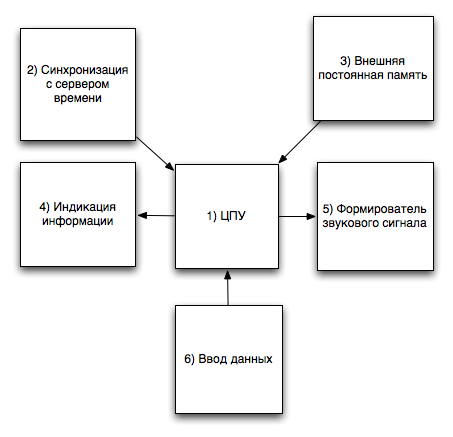
\includegraphics[bb=0 0 453 437, clip, scale=0.8]{funcd.png}}
	\caption{Фнкциональная структура}
	\label{img:funcd}
\end{figure}


\subsection{Детализация компонентов АСУ коптильной камеры}

\subsubsection{Датчики температуры коптильной камеры}

\subsubsection{Устройство подачи дыма и влаги коптильной камеры}

\subsubsection{Схема расположения датчиков и устройств регулирования в коптильной камере}

\subsubsection{Центральный вычислительный модуль устройства управления}
Центральное место в схеме занимает микроконтроллер atxmega128a3-au
TODO: описание функций выполняемых устройством

\subsubsection{Модуль индикации управляющего устройства}
\begin{par}
В качестве устройства индикации управляющего устройства в разрабатываемой АСУ должен использоваться TFT
ЖК-дисплей DST2001PH\cite{display} со встроенным драйвером ili9320 включённым в режиме system
i80 16-бит\cite{ili9320}.
Так как количество портов ввода-вывода на используемом микроконтролере достаточно, введение дополнительных узлов
расширяющих возможности ввода-вывода микроконтроллера --- не предусматривается.
\begin{figure}[h]
	\center{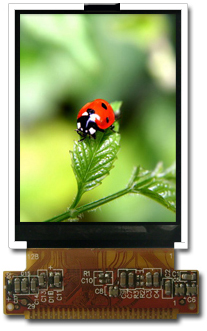
\includegraphics[bb=0 0 150 250, clip, scale=1.0]{ili9320.png}}
	\caption{Внешний вид TFT ЖК-дисплея DST2001PH}
	\label{img:iili9320}
\end{figure}
\end{par}

\begin{par}
В начальный момент работы, устройство должно погасить изображение на ЖК-дисплее и подготовить внутреннюю
память модуля индикации.
\end{par}

\subsubsection{Модуль ввода данных управляющего устройства}
\begin{par}
Модуль ввода данных пользователя выполнен на сенсорном экране ЖК-дисплея,
выполненного по 4-проводной схеме включения резистивного сенсорного экрана. Для
оцифровки значений плучаемых с сенсорного экрана должны использоваться АЦП\cite{avradc} центрального
микроконтроллера.
\end{par}

\begin{par}
В начальный момент работы устройства, после инициализация внутренней памяти ЖК-дисплея, должна быть
произведена процедура калибровки сенсорного экрана, а полученные коэффициенты далее должны быть
использованы для корректировки показаний снятых с сенсорного экрана. Это позволит отказаться
от дополнительной схемы температурной компенсации и статических калибровочных показателей,
и при этом устройство будет выдавать давольно стабильный результат,
так как эксплуатироваться устройство будет в условиях постоянной комнатной температуры,
а собственная рассеиваемая мощьность устройства не должна быть велика на столько, что бы
вносить ощутимую погрешность в показания.
\end{par}

\subsubsection{Модуль звукового оповещения}
\begin{par}
Звуковое оповещение о наступившем событии выполнено на широко распростонённой
микросхеме mc34119, включённой в стандартном режиме (рис. \ref{img:mc34119m}).
\begin{figure}[h]
	\center{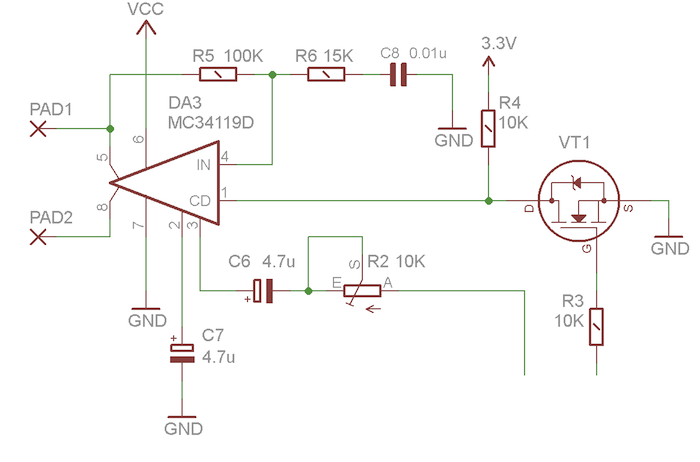
\includegraphics[bb=0 0 200 190, clip, scale=0.8]{mc34119.png}}
	\caption{Схема включения mc34119}
	\label{img:mc34119m}
\end{figure}
\end{par}

\begin{par}
В начальном состоянии на вход Chip Disable микросхемы mc34119 подавётся сигнал высокого уровня.
Это переводит микросхему в состояние низкого энергопотребления \cite{mc34119}.
\end{par}

\begin{par}
В момент наступления события будильника на вход Chip Disable микросхемы необходимо подать сигнал 
низкого уровня, выполнить задержку не менее 40 мс., необходимую для перевода микросхемы в
нормальное состояние, и затем подавать на неё вход сигнал с ЦАП центрального микроконтроллера.
Принципиальная схема ЦАП микроконтроллеров AVR семейства XMega приведена на рисунке \ref{img:avrdacp}.
\begin{figure}[h]
	\center{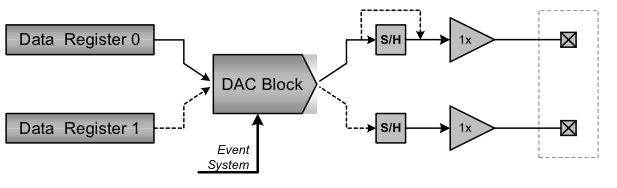
\includegraphics[bb=0 0 300 100, clip, scale=0.8]{avrdac.png}}
	\caption{Принципиальная схема ЦАП микроконтроллеров AVR семейства XMega}
	\label{img:avrdacp}
\end{figure}
\end{par}

\begin{par}
Для воспроизведения музыкального отрывка необходимо использовать нижние 8 бит 12-битного
ЦАП микроконтроллера. Опорное напряжение ЦАП микроконтроллера должно быть равно либо внутреннему
напряжению микроконтроллера 1 В, либо стабилизированному напряжению питания ($AV_{cc}$). Выбор того или иного
опорного напряжения ЦАП обусловливается параметрами динамика и необходимым уровнем громкости.
Для переодического получения данных и их переноса в буфер воспроизведения необходимо использовать
обработик прерывания таймера Timer 1 микроконтроллера. Частота срабатывания таймера выбирается
в соответствии с частотой дискретизации музыкального отрывка.
Механизм программирования ЦАП микроконтроллеров AVR семейства XMega детально описан в документации\cite{avrdac}.
\end{par}

\subsubsection{Модуль памяти устройства управления}
\begin{par}
В качестве устройства хранения звуковых отрывков используются энергонезависимые карты
памяти MicroSD. Применение этого вида памяти позволяет не пребегая к перепрограммированию устройства
вносить музыкальные фрагменты на карту с персонального компьютера, оснащённого модулем
чтения/записи карт MicroSD.
\end{par}

\begin{par}
Для воспроизведения звуковых отрывков центральным микроконтроллером должен быть
организован буфер воспроизведения, таким образом, что бы в случае отсутствия карты MicroSD или
сбоя доступа к ней, в него вносились записанные на этапе программирования данные EEPROM микроконтроллера.
\end{par}

\begin{par}
Для чтения данных карт памяти MicroSD должен использоваться SPI режим работы. Методика программирования
интерфейса SPI микроконтроллеров AVR семейства XMega дана в документации \cite{avrspi}.
\end{par}

\subsubsection{Модуль сетевого интерфейса устройства управления}

TODO: enc28j60 \\
TODO: UDP \\

\subsubsection{Контроллирующий удалённый сервис АСУ коптильной камеры}

TODO: erlang
TODO: OTP \\

